% Drawing 80/01-3 -- folder 80, batch 01, archive page 9 (PDF page 10).
% Transcription: grande figure occupant le haut et le milieu de la page : dans un cercle au crayon, un arrangement de neuf pseudo-droites, six droites $\Delta_A$, $\Delta_{A'}$, $\Delta_B$, $\Delta_{B'}$, $\Delta_C$, $\Delta_{C'}$ (deux à deux concourantes en trois points marqués près du bord) et trois courbes $D_A$, $D_B$, $D_C$ qui passent par le centre ; les extrémités portent ces étiquettes, les régions leur nombre de côtés ($3$, $4$, $5$, et $3'$, $4'$, $5'$), les points du centre les lettres $A$, $B$, $C$, $A'$, $B'$, $C'$, $L$, $M$, $N$, $L'$, $M'$, $N'$, $P$, $Q$, $R$, $P'$, $Q'$, $R'$ ; trois arcs du bord sont épaissis, trois autres en tirets
% Kind: arrangement of nine pseudo-lines in a disc. Method 2 (schematic redraw from the facsimile). Status: partial.
% Notes: Whole-page ink figure. The six lines Delta are straight and are drawn through three computed points: Delta_A and Delta_A' meet at the marked point on the right, Delta_B and Delta_B' at the one on the left, Delta_C and Delta_C' at the one below (heavy dots; the letter written at each is overwritten and is not set). The hexagon A, B', C, A', B, C' at the centre is formed by these six lines, each vertex the crossing of two of them, all computed. D_A, D_B, D_C are smooth curves through the points read on the page; P', P (D_A on Delta_C, Delta_C'), Q, Q' (D_C on Delta_A', Delta_A), R, R' (D_B on Delta_B', Delta_B) are computed on the lines. The pencil circle is drawn as a true circle (on the page it is free-hand and visible in parts). Heavy rim arcs between Delta_C' and Delta_C (top), Delta_A and Delta_A' (left), Delta_B' and Delta_B (right); the opposite short arcs dashed or dotted, as on the page. Editorial device: the centre, where his labels are 1 to 2 mm apart, is repeated below the figure enlarged 3.5 times (dotted frames), and the labels of the centre are set only there. Still differs: inside the hexagon the three curves cross within a few millimetres under ink blots; their paths there (the small central triangle, and on which side of each hexagon vertex a curve passes) are a reading, so the cells at the centre are not certified against his count 7 + 24 + 6 = 37 regions (which is the count of a simple arrangement of nine pseudo-lines); three blots at the centre and the overwritten letters at the three outer points are left out. His labels 3/3', 4/4', 5/5' are placed as read. Redrawn 2026-11-12 (issue 128): to check again.
% Coordinates: 1 unit = 1 mm = 1/100 of the crop width (bbox in page fractions: [0.09, 0.07, 0.92, 0.65]).
% Redrawn by Claude (claude-fable-5-2), issue #128, 2026-11-12; not checked by a human; not compiled (no TeX in the session).
% Rights: reproduces part of the work -- behind RENDER_TRANSCRIPTS, never published by itself.
\documentclass[tikz,border=3pt]{standalone}
\usepackage{amsmath,amssymb}
\usetikzlibrary{patterns,arrows.meta}
\tikzset{pencil/.style={black!45}, struck/.style={black!35}, mpt/.style={circle,draw,inner sep=1.3pt}, pt/.style={circle,fill,inner sep=0.9pt}, opt/.style={circle,draw,fill=white,inner sep=1.1pt}}
\begin{document}
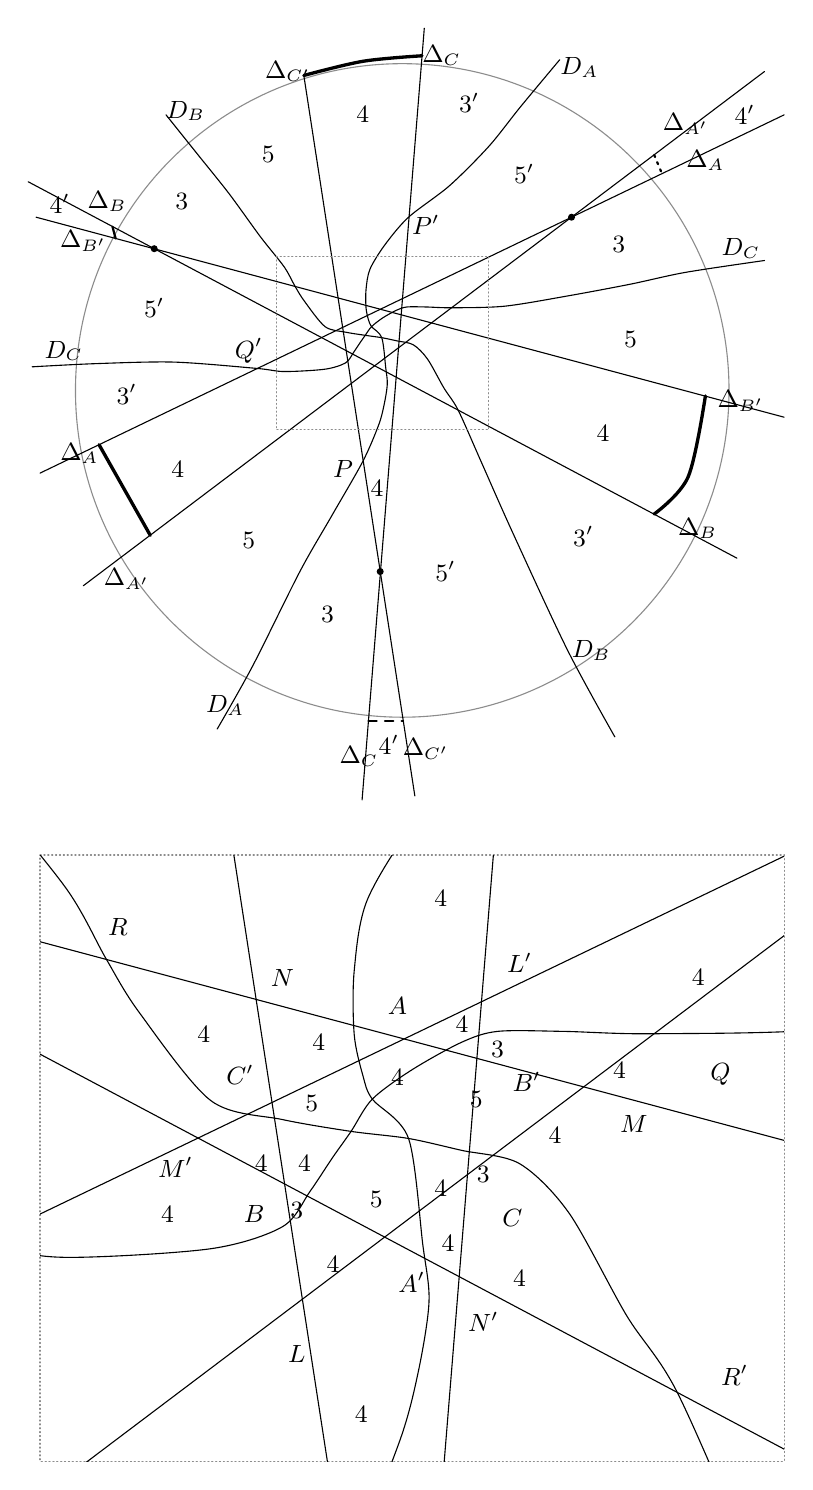
\begin{tikzpicture}[x=1mm,y=1mm,line cap=round,line join=round,font=\scriptsize]
\draw[pencil] (49,-47) circle[radius=41.5];
\draw (97.5,-12) -- (3,-57.5);
\draw (95,-6.5) -- (8.5,-71.8);
\draw (1.5,-20.5) -- (91.5,-68.3);
\draw (2.5,-25) -- (97.5,-50.4);
\draw (51.8,-1) -- (43.9,-99);
\draw (36.5,-7) -- (50.6,-98.5);
\draw plot[smooth, tension=0.5] coordinates {(69,-5) (64,-11) (60,-16) (55,-21) (49.8,-25) (46.8,-28.5) (44.9,-31.6) (44.4,-34.2) (44.4,-36.5) (44.7,-38) (45.1,-38.9) (46.4,-40.3) (46.9,-44.1) (47.1,-46.2) (46.7,-48.8) (46,-51.4) (44,-56) (40,-63) (36,-70) (30,-82) (25.5,-90)};
\draw plot[smooth, tension=0.5] coordinates {(19,-12) (23,-17) (27,-22) (31,-27.5) (34,-31.3) (35.4,-33.8) (36.6,-35.7) (39.2,-38.9) (41.8,-39.6) (44.3,-40) (46.4,-40.3) (48.3,-40.7) (50.4,-41.2) (52.2,-43) (54.3,-46.7) (56.1,-49.5) (59,-56) (63,-65) (70,-80) (76,-91)};
\draw plot[smooth, tension=0.5] coordinates {(2,-44) (10,-43.6) (20,-43.4) (30.5,-44.2) (34,-44.6) (39.2,-44.3) (41.8,-43.5) (42.8,-42.2) (43.6,-41) (44.3,-40) (45.1,-38.9) (46.5,-37.8) (48.3,-36.8) (49.6,-36.4) (52,-36.4) (55.3,-36.5) (62,-36.3) (70,-35) (78,-33.5) (85,-32) (95,-30.5)};
\draw[very thick] plot[smooth, tension=0.55] coordinates {(36.5,-7) (44,-5.2) (51.5,-4.5)};
\draw[very thick] (10.5,-53.9) -- (17,-65.4);
\draw[very thick] plot[smooth, tension=0.55] coordinates {(87.5,-47.7) (85.3,-58) (81,-62.7)};
\draw[thick,dashed] (44.7,-89) -- (49.1,-89);
\draw[thick,dotted] (81,-17.1) -- (82,-19.5);
\draw[thick] (12.2,-26.2) -- (12.6,-27.7);
\node[pt] at (70.5,-25) {};
\node[pt] at (17.5,-29) {};
\node[pt] at (46.2,-70) {};
\node[inner sep=1pt] at (34.5,-6.5) {\small $\Delta_{C'}$};
\node[inner sep=1pt] at (54,-4.5) {\small $\Delta_C$};
\node[inner sep=1pt] at (71.5,-6) {\small $D_A$};
\node[inner sep=1pt] at (85,-13.2) {\small $\Delta_{A'}$};
\node[inner sep=1pt] at (87.5,-17.8) {\small $\Delta_A$};
\node[inner sep=1pt] at (92.5,-12) {\small $4'$};
\node[inner sep=1pt] at (21.5,-11.5) {\small $D_B$};
\node[inner sep=1pt] at (5.5,-23.3) {\small $4'$};
\node[inner sep=1pt] at (11.5,-23) {\small $\Delta_B$};
\node[inner sep=1pt] at (8.5,-28) {\small $\Delta_{B'}$};
\node[inner sep=1pt] at (92,-29) {\small $D_C$};
\node[inner sep=1pt] at (6,-42) {\small $D_C$};
\node[inner sep=1pt] at (8,-55) {\small $\Delta_A$};
\node[inner sep=1pt] at (14,-71) {\small $\Delta_{A'}$};
\node[inner sep=1pt] at (92,-48.3) {\small $\Delta_{B'}$};
\node[inner sep=1pt] at (86.5,-64.5) {\small $\Delta_B$};
\node[inner sep=1pt] at (73,-80) {\small $D_B$};
\node[inner sep=1pt] at (26.5,-87) {\small $D_A$};
\node[inner sep=1pt] at (43.5,-93.5) {\small $\Delta_C$};
\node[inner sep=1pt] at (47.3,-92) {\small $4'$};
\node[inner sep=1pt] at (52,-92.5) {\small $\Delta_{C'}$};
\node[inner sep=1pt] at (44,-12) {\small $4$};
\node[inner sep=1pt] at (57.5,-10.5) {\small $3'$};
\node[inner sep=1pt] at (32,-17) {\small $5$};
\node[inner sep=1pt] at (64.5,-19.5) {\small $5'$};
\node[inner sep=1pt] at (21,-23) {\small $3$};
\node[inner sep=1pt] at (76.5,-28.5) {\small $3$};
\node[inner sep=1pt] at (17.5,-36.5) {\small $5'$};
\node[inner sep=1pt] at (78,-40.5) {\small $5$};
\node[inner sep=1pt] at (14,-47.5) {\small $3'$};
\node[inner sep=1pt] at (20.5,-57) {\small $4$};
\node[inner sep=1pt] at (74.5,-52.5) {\small $4$};
\node[inner sep=1pt] at (29.5,-66) {\small $5$};
\node[inner sep=1pt] at (72,-65.5) {\small $3'$};
\node[inner sep=1pt] at (54.5,-70) {\small $5'$};
\node[inner sep=1pt] at (39.5,-75.5) {\small $3$};
\node[inner sep=1pt] at (52,-26) {\small $P'$};
\node[inner sep=1pt] at (41.5,-57) {\small $P$};
\node[inner sep=1pt] at (29.5,-42) {\small $Q'$};
\node[inner sep=1pt] at (45.8,-59.5) {\small $4$};
\draw[pencil,densely dotted] (33,-30) -- (60,-30) -- (60,-52) -- (33,-52) -- (33,-30);
\draw[pencil,densely dotted] (3,-106) -- (97.5,-106) -- (97.5,-183) -- (3,-183) -- (3,-106);
\begin{scope}
\clip (3,-106) rectangle (97.5,-183);
\draw (228.8,-43) -- (-102,-202.1);
\draw (220,-23.8) -- (-82.8,-252.3);
\draw (-107.2,-72.8) -- (207.8,-240);
\draw (-103.8,-88.5) -- (228.8,-177.3);
\draw (68.8,-4.5) -- (41,-347.5);
\draw (15.2,-25.5) -- (64.6,-345.8);
\draw plot[smooth, tension=0.5] coordinates {(129,-18.5) (111.5,-39.5) (97.5,-57) (80,-74.5) (62,-88.5) (51.3,-100.8) (44.6,-111.6) (42.9,-120.7) (42.9,-128.8) (44,-134) (45.2,-137) (49.8,-142) (51.6,-155.4) (52.4,-162.7) (51,-171.8) (48.5,-180.9) (41.7,-197) (27.5,-221.5) (13.5,-246) (-7.5,-288) (-23.2,-316)};
\draw plot[smooth, tension=0.5] coordinates {(-46,-43) (-32,-60.5) (-18,-78) (-4,-97.2) (6.5,-110.5) (11.4,-119.2) (15.6,-126) (24.7,-137.2) (33.8,-139.6) (42.5,-141.1) (49.8,-142) (56.5,-143.5) (63.9,-145.2) (70.2,-151.5) (77.5,-164.5) (83.9,-174.2) (94,-197) (108,-228.5) (132.5,-281) (153.5,-319.5)};
\draw plot[smooth, tension=0.5] coordinates {(-105.5,-155) (-77.5,-153.6) (-42.5,-152.9) (-5.8,-155.8) (6.5,-157.1) (24.7,-156) (33.8,-153.2) (37.3,-148.7) (40.1,-144.5) (42.5,-141.1) (45.2,-137) (50.2,-133.3) (56.5,-129.8) (61.1,-128.4) (69.5,-128.4) (81,-128.7) (104.5,-128) (132.5,-123.5) (160.5,-118.2) (185,-113) (220,-107.8)};
\node[inner sep=1pt] at (53.9,-111.5) {\small $4$};
\node[inner sep=1pt] at (86.6,-121.6) {\small $4$};
\node[inner sep=1pt] at (76.6,-133.4) {\small $4$};
\node[inner sep=1pt] at (23.8,-128.8) {\small $4$};
\node[inner sep=1pt] at (38.4,-129.8) {\small $4$};
\node[inner sep=1pt] at (56.6,-127.5) {\small $4$};
\node[inner sep=1pt] at (48.4,-134.3) {\small $4$};
\node[inner sep=1pt] at (37.5,-137.5) {\small $5$};
\node[inner sep=1pt] at (58.4,-137) {\small $5$};
\node[inner sep=1pt] at (68.4,-141.6) {\small $4$};
\node[inner sep=1pt] at (31.1,-145.2) {\small $4$};
\node[inner sep=1pt] at (36.6,-145.2) {\small $4$};
\node[inner sep=1pt] at (45.7,-149.8) {\small $5$};
\node[inner sep=1pt] at (53.9,-148.4) {\small $4$};
\node[inner sep=1pt] at (59.3,-146.6) {\small $3$};
\node[inner sep=1pt] at (61.1,-130.7) {\small $3$};
\node[inner sep=1pt] at (35.6,-151.2) {\small $3$};
\node[inner sep=1pt] at (19.2,-151.6) {\small $4$};
\node[inner sep=1pt] at (40.2,-158) {\small $4$};
\node[inner sep=1pt] at (54.8,-155.3) {\small $4$};
\node[inner sep=1pt] at (63.9,-159.8) {\small $4$};
\node[inner sep=1pt] at (43.8,-177.1) {\small $4$};
\node[inner sep=1pt] at (33.8,-121.6) {\small $N$};
\node[inner sep=1pt] at (48.4,-125.2) {\small $A$};
\node[inner sep=1pt] at (63.9,-119.7) {\small $L'$};
\node[inner sep=1pt] at (12.9,-115.2) {\small $R$};
\node[inner sep=1pt] at (64.8,-134.8) {\small $B'$};
\node[inner sep=1pt] at (89.4,-133.9) {\small $Q$};
\node[inner sep=1pt] at (78.4,-140.2) {\small $M$};
\node[inner sep=1pt] at (20.2,-145.7) {\small $M'$};
\node[inner sep=1pt] at (28.4,-133.9) {\small $C'$};
\node[inner sep=1pt] at (30.2,-151.6) {\small $B$};
\node[inner sep=1pt] at (63,-152.1) {\small $C$};
\node[inner sep=1pt] at (50.2,-160.3) {\small $A'$};
\node[inner sep=1pt] at (59.3,-165.3) {\small $N'$};
\node[inner sep=1pt] at (35.6,-169.4) {\small $L$};
\node[inner sep=1pt] at (91.2,-172.1) {\small $R'$};
\end{scope}
\end{tikzpicture}
\end{document}
